\parindent=0em
\section{Dispositivos}
\noindent

%https://editeca.com/realidad-mixta/

Actualmente los dispositivos más utilizados para la realidad mixta son los cascos también conocidos como diademas, los cuales, vienen incorporados con: cámaras, sensores infrarrojos, micrófonos y acelerómetros entre otros. \\\\Estos dispositivos se pueden clasificar en dos grupos:

\begin{itemize}
    \item \textbf{Dispositivos holográficos:} Se trata de aquellos que crean imágenes tridimensionales basadas en el empleo de la luz (hologramas) haciendo que el contenido parezca que está realmente en el mundo físico.
    
    \item \textbf{Dispositivos envolventes:} Estos dispositivos son capaces de remplazar el mundo físico por una experiencia digital, bloqueando el entorno físico.
    
\end{itemize}

Por otra parte, los teléfonos móviles están empezando a ganar importancia en el sector de la realidad mixta. Según un estudio realizado por Sam Barker \cite{juniperArMrmoney} , la aparición de las redes de  5G y los avances del Edge Computing acelerarán el desarrollo de la tecnología de realidad mixta en móviles llegando a alcanzar un mercado de 43 billones de dólares en el año 2024, a diferencia de los 8 billones alcanzados en 2019.

\parindent=0em
\subsection{Hololens 2}
\label{HoloLens2Dispositivo}
\noindent

Las \textit{HoloLens 2} (figura~\ref{fig:vistasHoloLens2}) son un casco desarrollado por \textit{Microsoft} que salió al mercado en 2019. Es un dispositivo dotado de tecnología de \textit{eye tracking} y \textit{hand tracking} capaz de detectar las dos manos, esto añade un extra de inmersión a la experiencia y de comodidad ya que no se necesitan mandos para manejarlo y se pueden tener las manos libres. Respecto a los sensores, goza de acelerómetro, giroscopio y magnetómetro para medir la velocidad, orientación y fuerzas gravitacionales del dispositivo.\\


\begin{figure}[htbp]
\centering
    \hspace{-4mm}
    \begin{minipage}{0.5\textwidth}
        \centering
        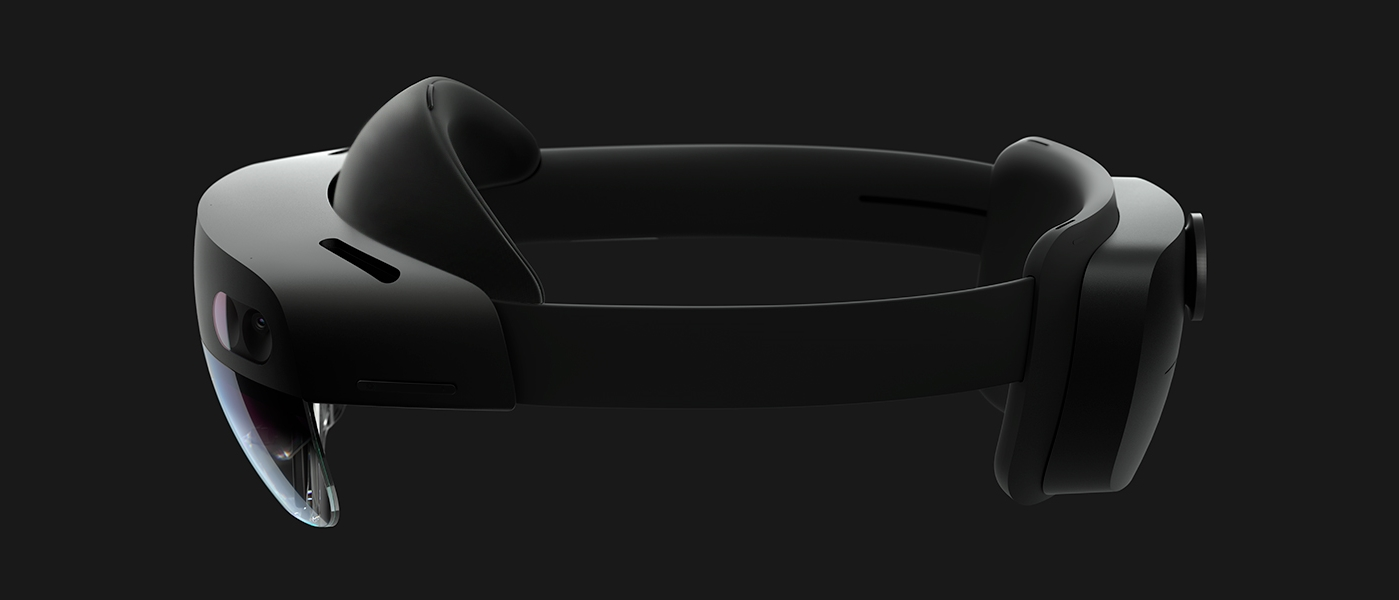
\includegraphics[scale=0.2]{Images/Estado del arte/hololens2_2.jpeg}\\
        (a) Vista lateral.
    \end{minipage}
    \begin{minipage}{0.5\textwidth}
        \centering
        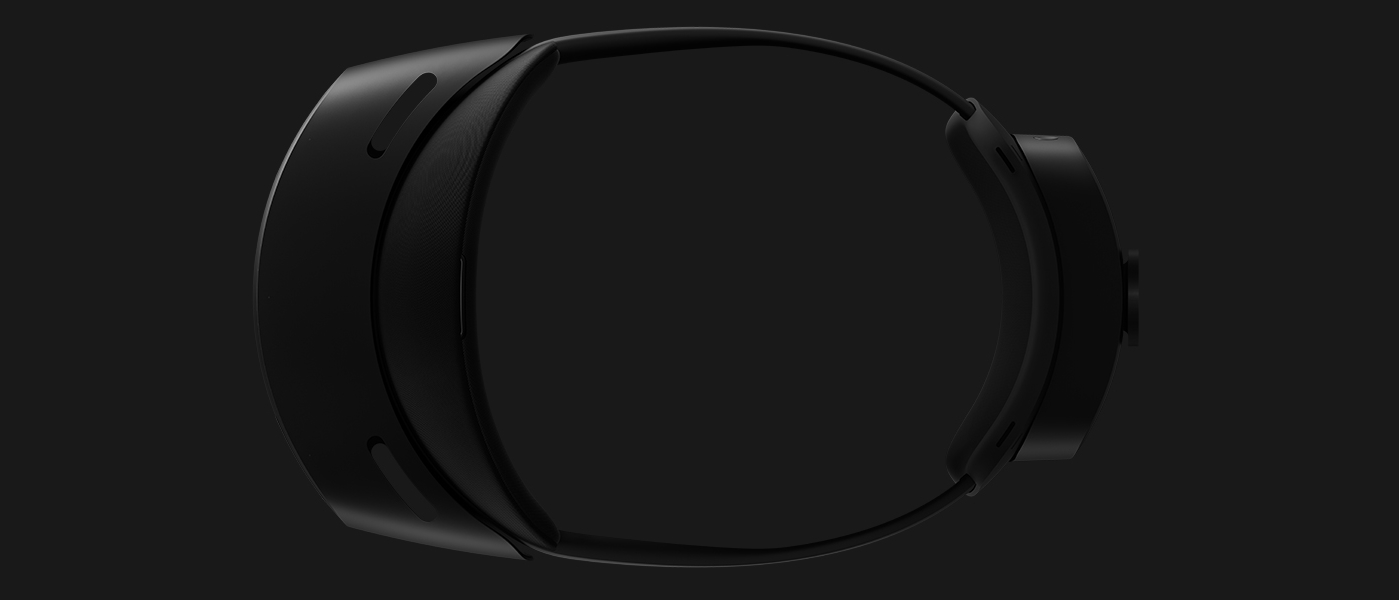
\includegraphics[scale=0.2]{Images/Estado del arte/hololens2_3.jpeg}\\
       (b) Vista superior.
    \end{minipage}\\
    \caption{Vistas de las Microsoft HoloLens 2\textsuperscript{\ref{hololens2footer}}.}
    \label{fig:vistasHoloLens2}
\end{figure}


Las \textit{Hololens 2} funcionan de forma independiente ya que tienen integrado su propio procesador y utilizan una batería recargable con una autonomía de entre 2 y 3 horas, además, permiten capturar el movimiento y los giros del usuario gracias a su control de \textit{6DoF}. Por otra parte, respecto a la conectividad, este \textit{HMD} tiene \textit{WiFi}, \textit{bluetooth} y permite conexiones mediante un \textit{USB} tipo C. Por ejemplo, se puede utilizar la conexión \textit{WiFi} para navegar por internet (a través del navegador \textit{Microsoft Edge} incorporado en las gafas) o para conectarse a reuniones en línea con otros usuarios de las mismas gafas.\\

Del mismo modo, este casco  está diseñado con un sistema ergonómico de tal forma que no hay necesidad de quitarse las gafas, ya que se puede colocar directamente sobre ellas (figura~\ref{fig:hololensErgonomicas}).\\


\begin{figure}[H]
    \centering
    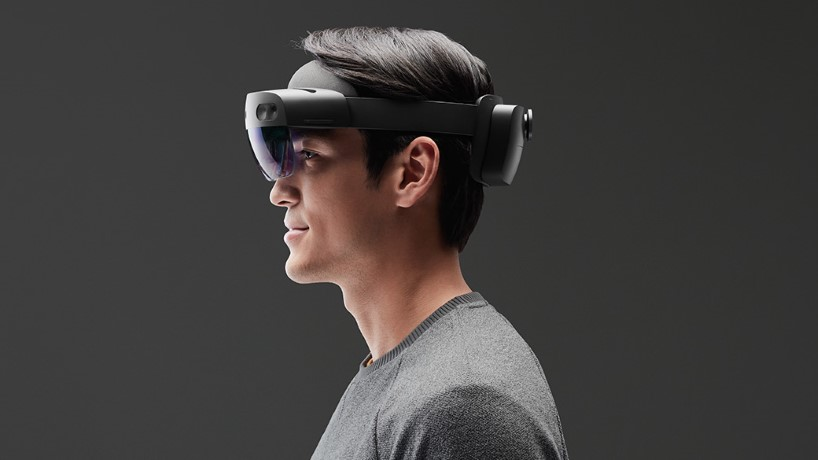
\includegraphics[scale=0.35]{Images/Estado del arte/hololens2_1.jpeg}
     \caption{Diseño ergonómico del dispositivo\textsuperscript{\ref{hololens2footer}}.
  }
  \label{fig:hololensErgonomicas}
\end{figure}


Para finalizar, este \textit{HMD} tiene un \textit{FOV} de 43º, una resolución de 2.048×1.080 píxeles por ojo (4.096x1.080 en combinación) y una \textit{IPD} que se ajusta automáticamente según la posición de los ojos que es detectada por un sensor \textit{IPD}, asimismo, tiene un sensor de~1~Megapíxel de profundidad \textit{ToF} (del inglés Time of Flight, calcula distancias entre objetos en función a la distancia que tarda la emisión y recepción de un haz de luz infrarrojo) y un peso de 566 gramos.  


%https://www.microsoft.com/es-es/hololens/hardware



\parindent=0em
\subsection{HMD Odyssey+}
\label{sec:odyssey}
\noindent

%https://www.samsung.com/hk_en/news/product/reality-headset-hmd-odyssey-plus/

El casco \textit{HDM Odyssey+} (figura~\ref{fig:hdmOdysseyVista}) es un dispositivo desarrollado por la empresa \textit{Samsung} que salió al mercado en 2018, no es un casco independiente ya que requiere estar conectado a un ordenador compatible con la plataforma \textit{Windows Mixed Reality} para funcionar, se conecta al ordenador mediante un cable \textit{HDMI}~2.0 y un \textit{USB}~3.0.

\begin{figure}[h]
    \centering
    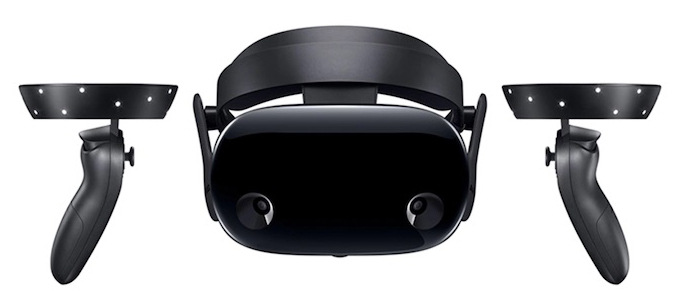
\includegraphics[scale=0.6]{Images/Estado del arte/samsungOdysseyplus.jpg}
    \caption{HDM Odyssey+ dispositivo al completo.}
    \label{fig:hdmOdysseyVista}
\end{figure}

En cuanto a la parte de monitorización de la imagen, este casco tiene una resolución de 1.440 x 1.600 píxeles por ojo, un total de 2.880 x 1.600 píxeles combinando los dos ojos, además, el \textit{Field of View} abarca un total de 110º. Este dispositivo no posee tecnología de \textit{hand tracking} (por lo que controla el movimiento de manos con dos mandos que funcionan con pilas) y tampoco tiene \textit{eye tracking}, en cambio, destaca por tener dos sensores \textit{6DoF} frente al único que tiene, por ejemplo, las \textit{Hololens~2} (sección~\ref{HoloLens2Dispositivo}).\\

Por otra parte, está dotado de sensores como acelerómetro, giroscopio, brújula y sensor de proximidad (este último se utiliza para saber en qué momento se lleva puesto el casco), del mismo modo, posee una diadema que se puede  modificar para ajustar el casco a la cabeza de cada individuo, sin embargo, este dispositivo no está diseñado para ser utilizado con gafas.\\ 

Por último, tiene un sensor que ajusta automáticamente la \textit{IPD}, conexión \textit{bluetooth} y un peso total de 644g teniendo en cuenta solo el \textit{HMD} y un añadido de 176g si se cuenta el peso del cable.


\footnotetext[1]{
\label{hdmOdysseyfooter}{Imagen de la HDMOdyssey+: \url{https://www.samsung.com/us/computing/hmd/windows-mixed-reality/hmd-odyssey-windows-mixed-reality-headset-xe800zba-hc1us/}.}}

\footnotetext[1]{
\label{hdmOdysseyfooter}{Especificaciones de la HDMOdyssey+: \url{https://www.microsoft.com/en-us/p/samsung-hmd-odyssey/8n2d0nk20p8m?cid=msft_web_collection&activetab=pivot:techspecstab}.}}
\parindent=0em
\subsection{Magic Leap One}
\noindent

El dispositivo \textit{Magic Leap One}\textsuperscript{\ref{magicLeaponeFotterSpecs}} fue lanzado al mercado el 8 de Agosto de 2018 de manos de la compañía Magic Leap a un precio inicial de 2,295 dólares exclusivamente en Chicago, Los Ángeles, Miami, Nueva York, San Francisco y Seattle .\\

En el ámbito técnico este casco destaca por su ligero peso de 316 gramos frente a los 566 gramos de la HoloLens 2 (sección \ref{HoloLens2Dispositivo}), posee un sistema 6DoF para el tracking, conectividad vía Bluetooth 4.2, WiFi o USB tipo C.\\

\begin{figure}[htbp]
\centering
    \hspace{-4mm}
    \begin{minipage}{0.5\textwidth}
        \centering
        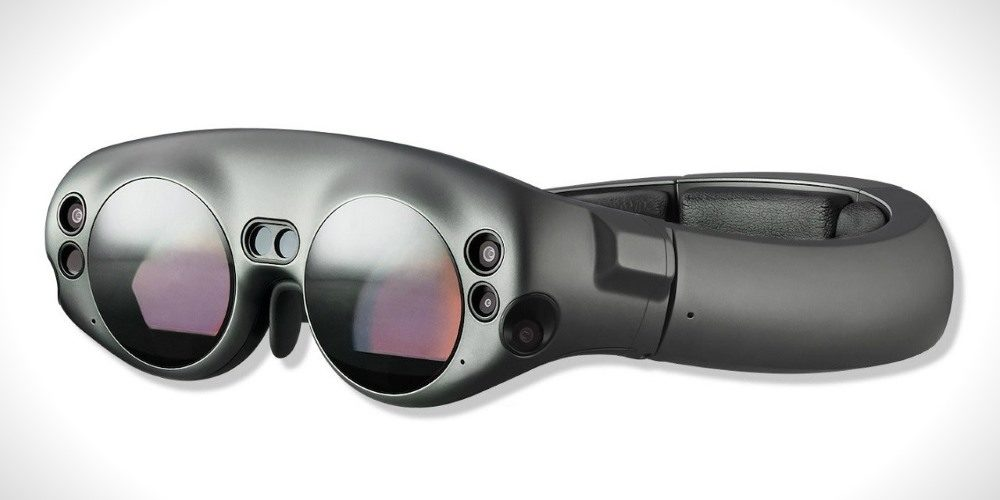
\includegraphics[scale=0.8]{Images/Estado del arte/magicleapone1.jpg}\\
        (a) Vista del casco completo
    \end{minipage}
    \begin{minipage}{0.5\textwidth}
        \centering
        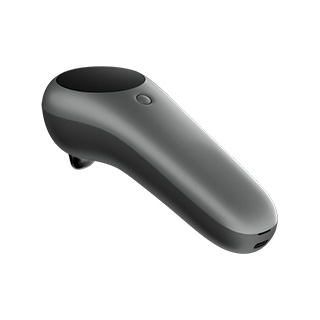
\includegraphics[scale=0.3]{Images/Estado del arte/magicleapone2.jpg}\\
       (b) Vista del mando
    \end{minipage}\\
    \caption{Dispositivo completo de las Magic Leap One\textsuperscript{\ref{magicLeaponeFotterImages}}.}
    \label{fig:vistasMagicLeapnOne}
\end{figure}

Por otro lado, utiliza una CPU (Unidad Central de Procesamiento) dos núcleos Denver 2.0 64-bit y cuatro núcleos ARM Cortex A57 64-bit, una Nvidia Pascal de 256 núcleos CUDA para la GPU (Unidad de Procesamiento Gráfico), tiene 128 Gigabytes como capacidad de almacenamiento y, por último, una batería de litio recargable que permite un uso continuado de 3 horas. 


%https://www.businessinsider.com/magic-leap-one-creator-edition-price-specifications-battery-life-release-date-2018-8?IR=T


\footnotetext[1]{
\label{magicLeaponeFotterSpecs}{Especificaciones obtenidas de \url{https://www.businessinsider.com/magic-leap-one-creator-edition-price-specifications-battery-life-release-date-2018-8?IR=T}.}}

\footnotetext[1]{
\label{magicLeaponeFotterImages}{Imágenes sacadas de \url{https://www.estiloextra.net/magic-leap-one-las-nuevas-y-prometedoras-gafas-de-realidad-aumentada/}.}}

\parindent=0em
\subsection{DAQRI Smart Helmet}
\label{subsec:DAQRISMART}
\noindent

%https://www.linkedin.com/pulse/daqri-smart-helmet-closer-look-nathan-gaydhani

El \textit{DAQRI Smart Helmet} (figura~\ref{fig:vistaDAQRIHelmet}) es un HMD enfocado al uso industrial, está formado por un dispositivo de realidad mixta sin cables integrado en un casco duro (cascos utilizados por ejemplo en la construcción). Ya que está pensado para un uso industrial está dotado de 4 cámaras para poder capturar todo el entorno, es decir, abarcar 360\degree .\\

\begin{figure}[H]
    \centering
    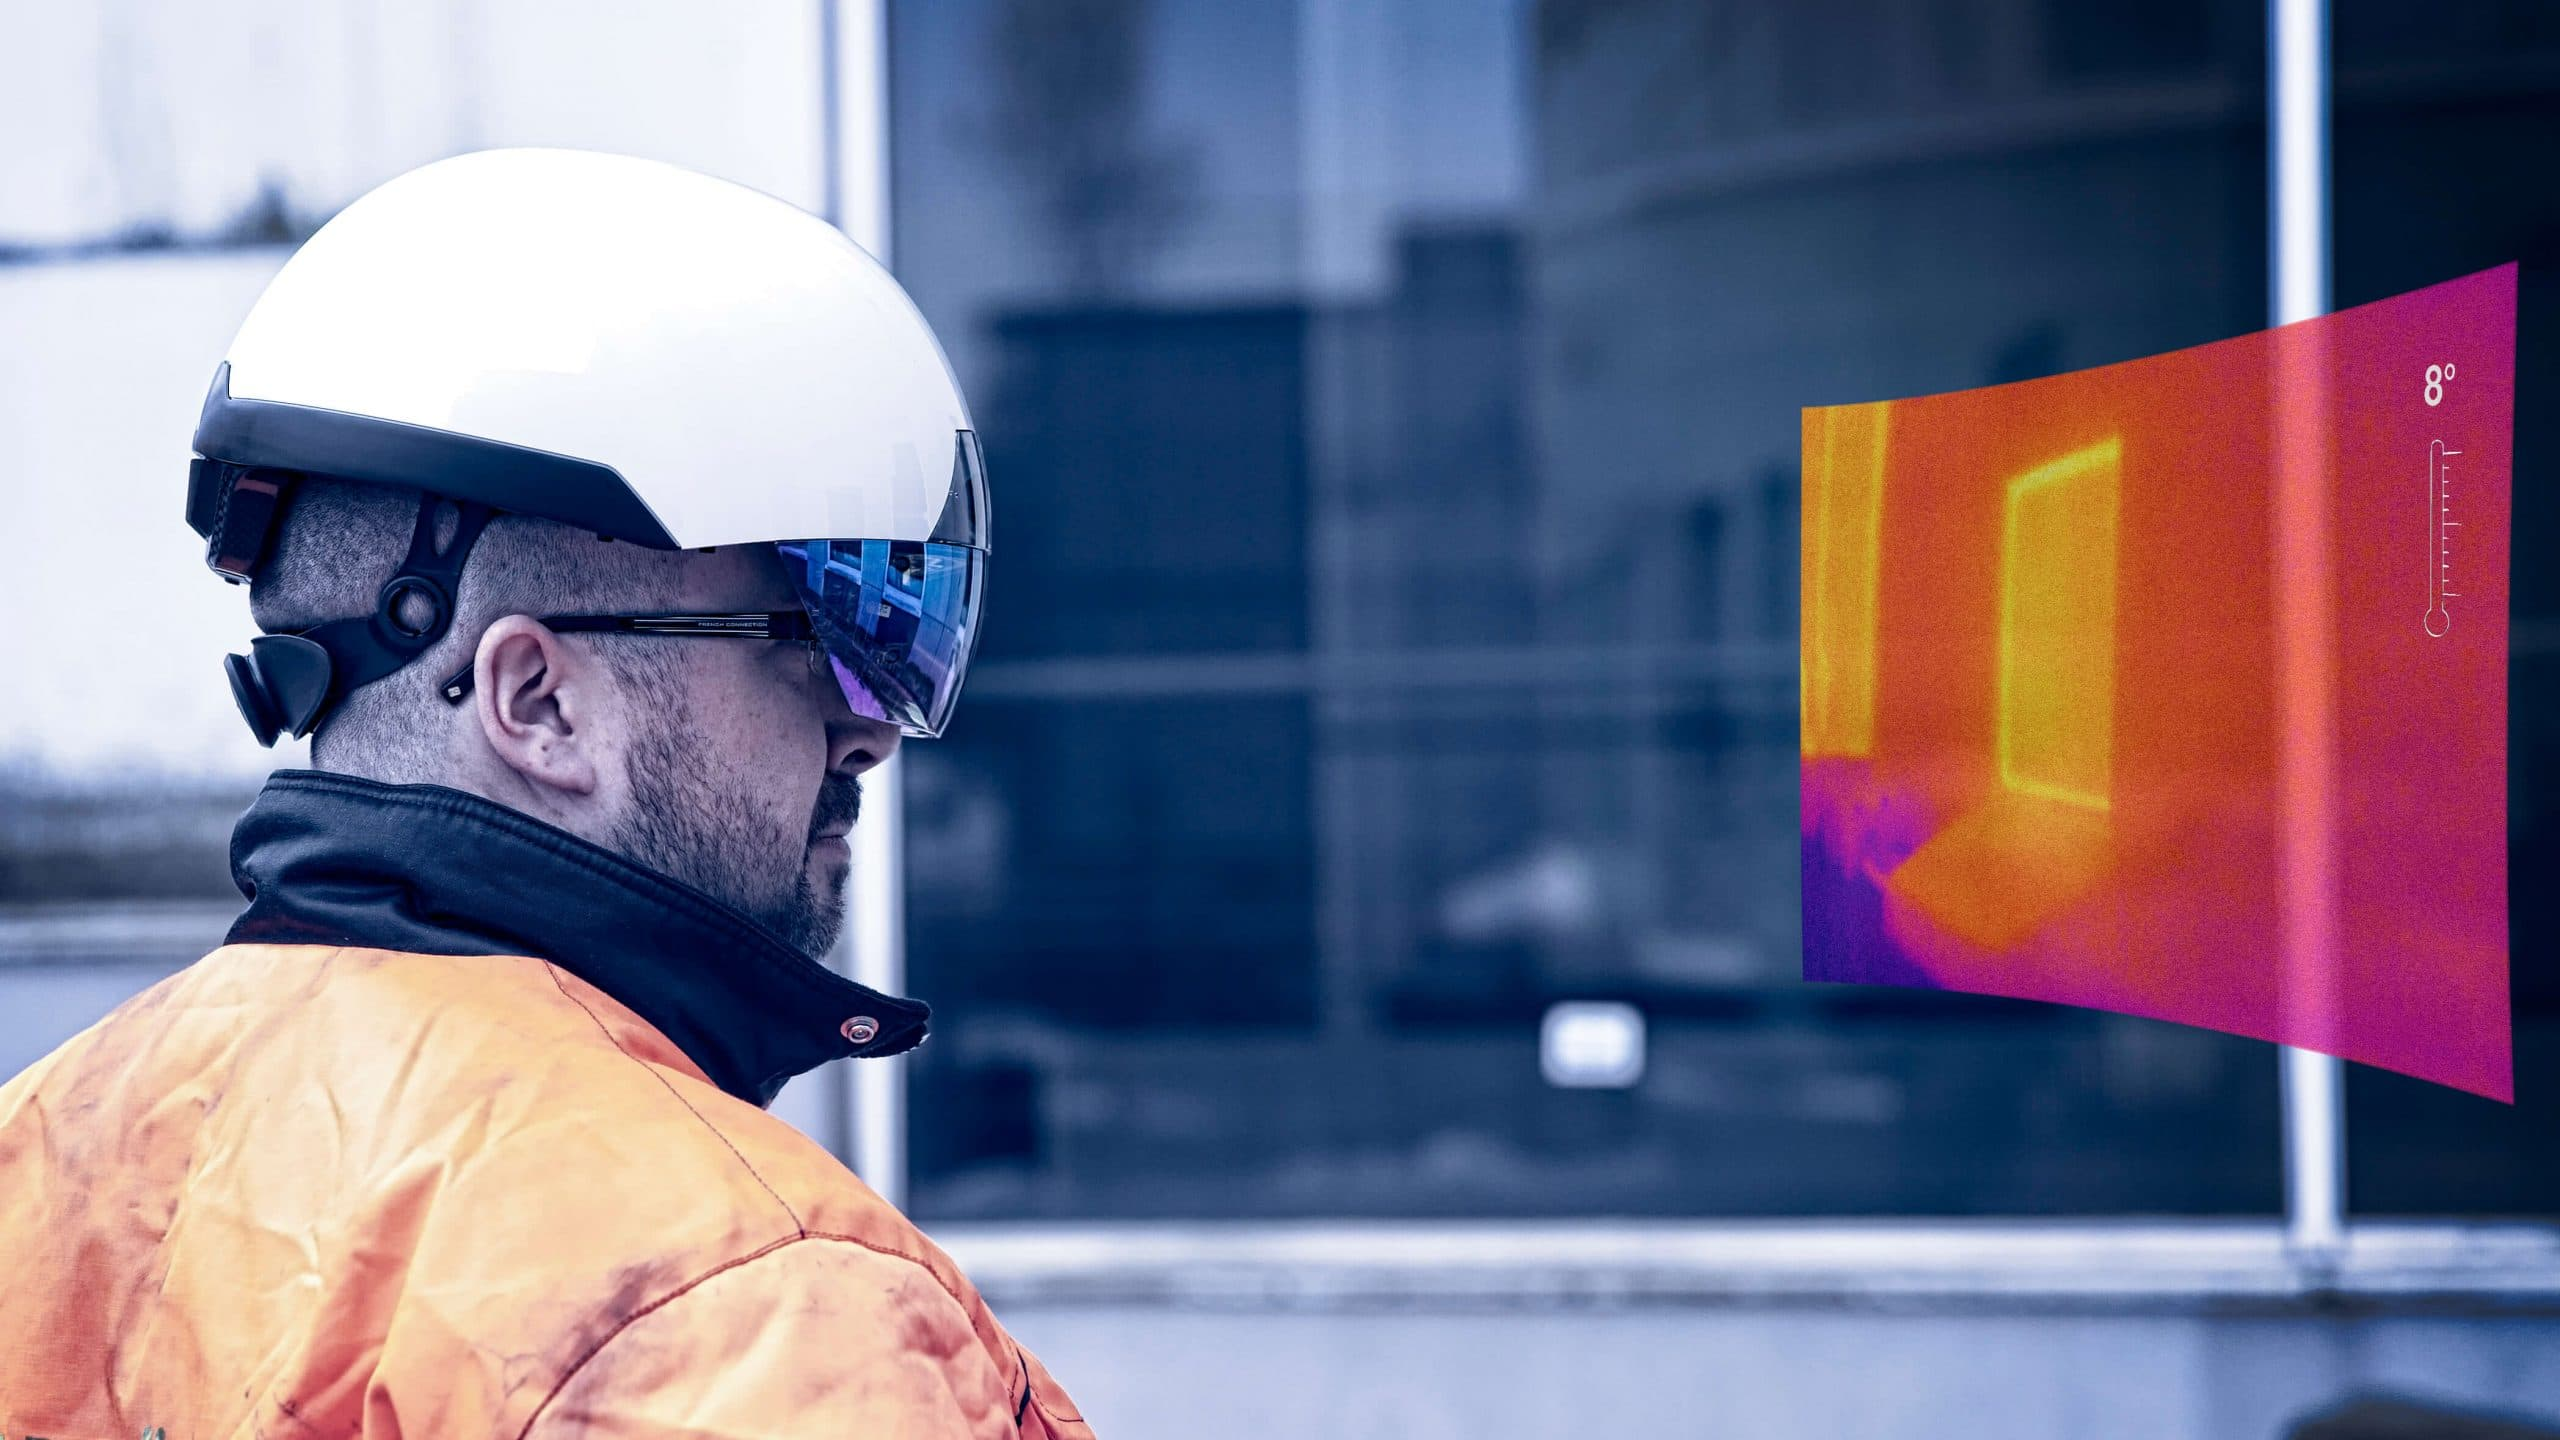
\includegraphics[scale=0.12]{Images/Estado del arte/daqrihelmet.jpg}
    \caption[Vista del \textit{DAQRI Smart Helmet}]{Vista del \textit{DAQRI Smart Helmet}\footnotemark.}
    \label{fig:vistaDAQRIHelmet}
\end{figure}

\footnotetext{Fuente: \href{https://www.stereoscape.com/blog/2017/04/25/daqri-smart-helmet-so-much-more-than-a-helmet/}{\nolinkurl{https://www.stereoscape.com/blog/2017/04/25/daqri-smart-helmet}}}


Con el objetivo de proteger al usuario en entornos industriales peligrosos, el dispositivo cuenta con una cámara termográfica (para poder controlar lugares potencialmente peligrosos debido a su temperatura) y barómetro para poder medir la presión del entorno.\\

Para el seguimiento, el \textit{DAQRI Smart Helmet} utiliza la tecnología SLAM y posee 6DoF para el movimiento y los giros del usuario. Del mismo modo, ya que el objetivo final es proteger al usuario, el dispositivo cuenta con reconocimiento de órdenes por voz y de control de movimientos de la cabeza para manejar el HMD, de esta forma se pueden tener las manos libres.\\


Finalmente, cabe recalcar que el casco goza de procesadores y un sistema operativo Android para ser totalmente independiente, también, utiliza unas baterías intercambiables de 5.700 miliamperios por hora y dispone de conectividad WiFi para poder comunicarse por vídeo en tiempo real remotamente con otros usuarios. El casco tiene un peso total de 1 kilo y~500 gramos y su precio actual es de~15.000 dólares.

%\footnotetext{\label{daqriImagefooter}{Imagenes obtenida de: %\url{https://www.stereoscape.com/blog/2017/04/25/daqri-smart-helmet-so-m%uch-more-than-a-helmet/}.}}


